\section{Results}
\label{sec:oct_results}
We present the descriptive statistics of the training and testing sets in \Cref{tab:dataset}. The OCT data comes from the Dept. of Ophthalmology, Bern University Hospital (Switzerland) and was acquired using the Heidelberg Spectralis system. The resolution of all slices is 496×512 pixels. The training and testing sets are similar in terms of pathologies, with the main difference being  the granularity of the annotations: the training dataset only contains slice-level annotations for two biological markers, while the testing dataset includes additional ETDRS rings information at 1mm, 3mm and 6mm per slice. In addition, a subset of the testing dataset has been manually segmented. Therefore, pixel-wise annotations for IRF and SRF are also available in 54 volumes (2’646 OCT slices). None of the patients in this test data are present in the training data. The distribution of IRF and SRF occurrences in the testing dataset is given in \Cref{tab:results}.

\noindent
\begin{table*}[t]
\centering
\caption{Dataset description}
\label{tab:dataset}
\begin{tabular}{p{4cm}p{5.5cm}p{5.5cm}}
\toprule
 & Training dataset & Testing dataset \\ \midrule
Number of patients & 433 & 189 \\
Number of eyes & 460 & 322 \\
Number of slices & 22’723 & 28'322 \\
Present pathologies & Diabetic retinopathy with and without Diabetic Macular Edema (DME), and early, intermediate, and late AMD & DME \\
Annotations & Slice-level annotations for IRF and SRF & Slice-level SRF and IRF presence   annotations for the ETDRS rings at 1mm, 3mm, and 6mm \\ \bottomrule
\end{tabular}

\end{table*}

\subsection{Implementation and baselines}
The backbone model of our method is an EfficientNet-b4~\sidecite{Tan2019} with ImageNet-initialized weights. As a preliminary step, we train the network alone in the task of IRF and SRF multilabel classification to produce slice-level predictions, and then fine-tune the entire model as described in the Methods section with the loss function of Eq. 5. We use a batch size of 32 slices\sidenote{A batch size of 32 means that we are using 32 slices and their flipped version for $\ell_3$.}, SGD with momentum of 0.9 and a base learning rate of $5\cdot10^{-3}$ which is scaled by 0.99 after every epoch. The feature map z of EfficientNet-b4 is sized 1792×16×16. We perform maximum and average pooling per column to produce C=16 descriptor vectors $d_c$ of dimension $2D_z=3584$, which are subsequently processed by the MLP to get 16 column-level predictions. The MLP itself consists of a single linear layer with 2 outputs for SRF and IRF, followed by a sigmoid activation. The column-level predictions are then mapped to ring-level predictions as explained at the end of the Methods section.

While there are no direct existing baselines for localization of OCT biological markers with weak annotations, we compare our method to the following alternative baselines:
\begin{itemize}
    \item \textbf{Masking} At test time, we mask the slice regions to only reveal relevant ETDRS rings and feed this to an EfficientNet trained on the slice-level detection task (as above). This masking has been done by replacing all pixels in the region to 0.
    
    \item \textbf{Masking with partial convolutions (PartConvs)} As in the \textbf{Masking} baseline but replacing all convolutional layers by partial convolutions~\sidecite{Liuc}, except for those in the squeeze and excitation blocks~\sidecite{Hu2019}, so to ignore masked regions.
    
    \item \textbf{Grad-CAM} We use Grad-CAM~\sidecite{Selvaraju2019} to build a 16×16 heatmap for each output variable and pick the maximum value of each column. This serves as a column-level measurement of the presence of SRF and IRF. We use the pre-trained EfficientNet to obtain the final ring-level predictions by applying the same post-processing mapping explained at the end of the Methods section.

    \item \textbf{MS-CAM}~\sidecite{ma2020} this approach consists of two stages: first, the activations of the different features of the resolutions are combined with Grad-CAM++~\sidecite{chattopadhay2018grad} to obtain a pixel-wise segmentation. Second, these segmentations are refined using Conditional Random Fields on the en-face projection image\sidedef{En-face Projection}{\jgt{TODO}}. We reproduced the first stage and converted the resulting pixel-wise segmentation into rings. 
\end{itemize}

All methods were implemented using PyTorch. Our method and the baselines were trained for 10 epochs.

\subsection{Localization results}
\marginfig{Figures/example_columns.pdf}{Outputs of our method and baselines. We show the slice number (bottom right) and in which ring the marker can be found (top row). Incorrect detections are highlighted in red.}{fig:examples}

\Cref{tab:results} reports the performance of all methods in terms of AUC ROC and Average Precision (AP). Our method achieves the highest ROC-AUC and AP for every marker and ETDRS ring. The improvement is particularly notable for 6mm SRF, where our method doubles the performance of other baselines in AP. \Cref{fig:results_curves} compares our method's ROC and Precision-Recall curves and the PartConvs baseline throughout the three ETDRS rings. \Cref{tab:results} also shows the occurrence of both biological markers in each one of the rings. IRF is present in 51.5\% of the images in the testing set, while SRF is scarcer and present in only 2.8\%. This imbalance is further exacerbated in the ring annotations: as depicted in Figure 1, where the 6mm ring is present in all the B-Scans. However, 38.4\% have IRF in the 6mm ring, but only 0.4\% have SRF. This is explained by the fact that SRF is unlikely to be found in the outer rings, leading to a lower number of occurrences in the test set than IRF. 

\noindent
\begin{table*}[t]
\centering
\caption{Comparison of the proposed method to evaluated baselines in terms of AUC ROC and AP on the {\bf Location dataset} for all markers on the entire slice and in the different ETDRS rings. The first row indicates the occurrences of each marker in this dataset.\label{tab:results}}
\begin{tabular}{@{}TrSSSSSS|SS@{}}
\cmidrule(l){3-10}
\multicolumn{1}{l}{}          & \multicolumn{1}{l}{}           & \multicolumn{2}{c}{\textbf{1mm}} & \multicolumn{2}{c}{\textbf{3mm}} & \multicolumn{2}{c}{\textbf{6mm}}                   & \multicolumn{2}{c}{\textbf{Present}} \\ \cmidrule(l){3-10} 
\multicolumn{1}{l}{}          & \multicolumn{1}{l}{}           & \textbf{IRF}    & \textbf{SRF}   & \textbf{IRF}    & \textbf{SRF}   & \textbf{IRF}  & \multicolumn{1}{c|}{\textbf{SRF}}  & \textbf{IRF}      & \textbf{SRF}     \\ \midrule
\multicolumn{1}{l}{}          & \multicolumn{1}{r|}{Occ. (\%)} & 13.0            & 2.1            & 31.9            & 1.2            & 38.4          & \multicolumn{1}{c|}{0.4}           & 51.5              & 2.8              \\ \midrule
\multirow{4}{*}{\textbf{AUC}} & \multicolumn{1}{r|}{Masking}   & 92.6            & 91.7           & 89.6            & 81.6           & 92.7          & \multicolumn{1}{c|}{66.7}          & 96.5              & 96.2             \\
& \multicolumn{1}{r|}{PartConvs}    & \textbf{93.2}   & 94.1           & 90.2            & 89.8           & 91.7          & \multicolumn{1}{c|}{74.9}          & 94.2              & 89.7             \\
& \multicolumn{1}{r|}{Grad-CAM}  & 85.2            & 87.3           & 89.2            & 76.0           & 89.4          & \multicolumn{1}{c|}{64.6}          & 96.5              & 96.2             \\
& \multicolumn{1}{r|}{MS-CAM~\cite{ma2020}}  & 55.7            & 70.4           & 57.5            & 64.1           & 55.0          & \multicolumn{1}{c|}{56.0}           & 56.0              & 53.7            \\
& \multicolumn{1}{r|}{\bf{Ours}}  & 90.6            & \textbf{97.5}  & \textbf{92.7}   & \textbf{93.8}  & \textbf{94.1} & \multicolumn{1}{c|}{\textbf{95.1}} & \textbf{97.2}     & \textbf{97.7}    \\ \midrule
\multirow{4}{*}{\textbf{AP}}  & \multicolumn{1}{r|}{Masking}   & 76.9            & 48.3           & 84.2            & 17.2           & \textbf{88.5} & \multicolumn{1}{c|}{5.6}           & 96.1              & 72.3             \\
& \multicolumn{1}{r|}{PartConvs}    & 81.8            & 60.5           & 85.2            & 21.4           & 88.1          & \multicolumn{1}{c|}{8.2}           & 94.2              & 38.5             \\
& \multicolumn{1}{r|}{Grad-CAM}  & 88.2            & 68.4           & 86.9            & 25.4           & 78.7          & \multicolumn{1}{c|}{7.4}           & 96.1              & 72.3             \\

& \multicolumn{1}{r|}{MS-CAM~\cite{ma2020}}  & 70.3            & 38.5           & 64.1            & 14.4           & 54.3          & \multicolumn{1}{c|}{1.6}           & 55.6              & 3.1             \\

& \multicolumn{1}{r|}{\bf Ours}  & \textbf{92.1}   & \textbf{86.6}  & \textbf{93.7}   & \textbf{52.7}  & 88.3          & \multicolumn{1}{c|}{\textbf{19.1}} & \textbf{96.8}     & \textbf{77.9}    \\ \bottomrule
\end{tabular}
%\caption{Comparison of the proposed method to evaluated baselines in terms of AUC ROC and AP on the {\bf Location dataset} for all markers on the entire slice and in the different ETDRS rings. The first row indicates the occurrences of each marker in this dataset.
%\label{tab:results}
\end{table*}

\textfig[t]{1}{Figures/all_plots.pdf}{ROC and Precision-Recall curves for both markers and rings with our proposed method on the testing dataset (solid lines). Results are compared to Partial Convolutions (dashed lines) on the same dataset.
}{fig:results_curves}

\Cref{fig:examples} illustrates the performance of the different methods in several cases. \jgt{We provide additional cases in Fig. S1 in the supplementary material.}

%\begin{figure}[t]
%\centering
%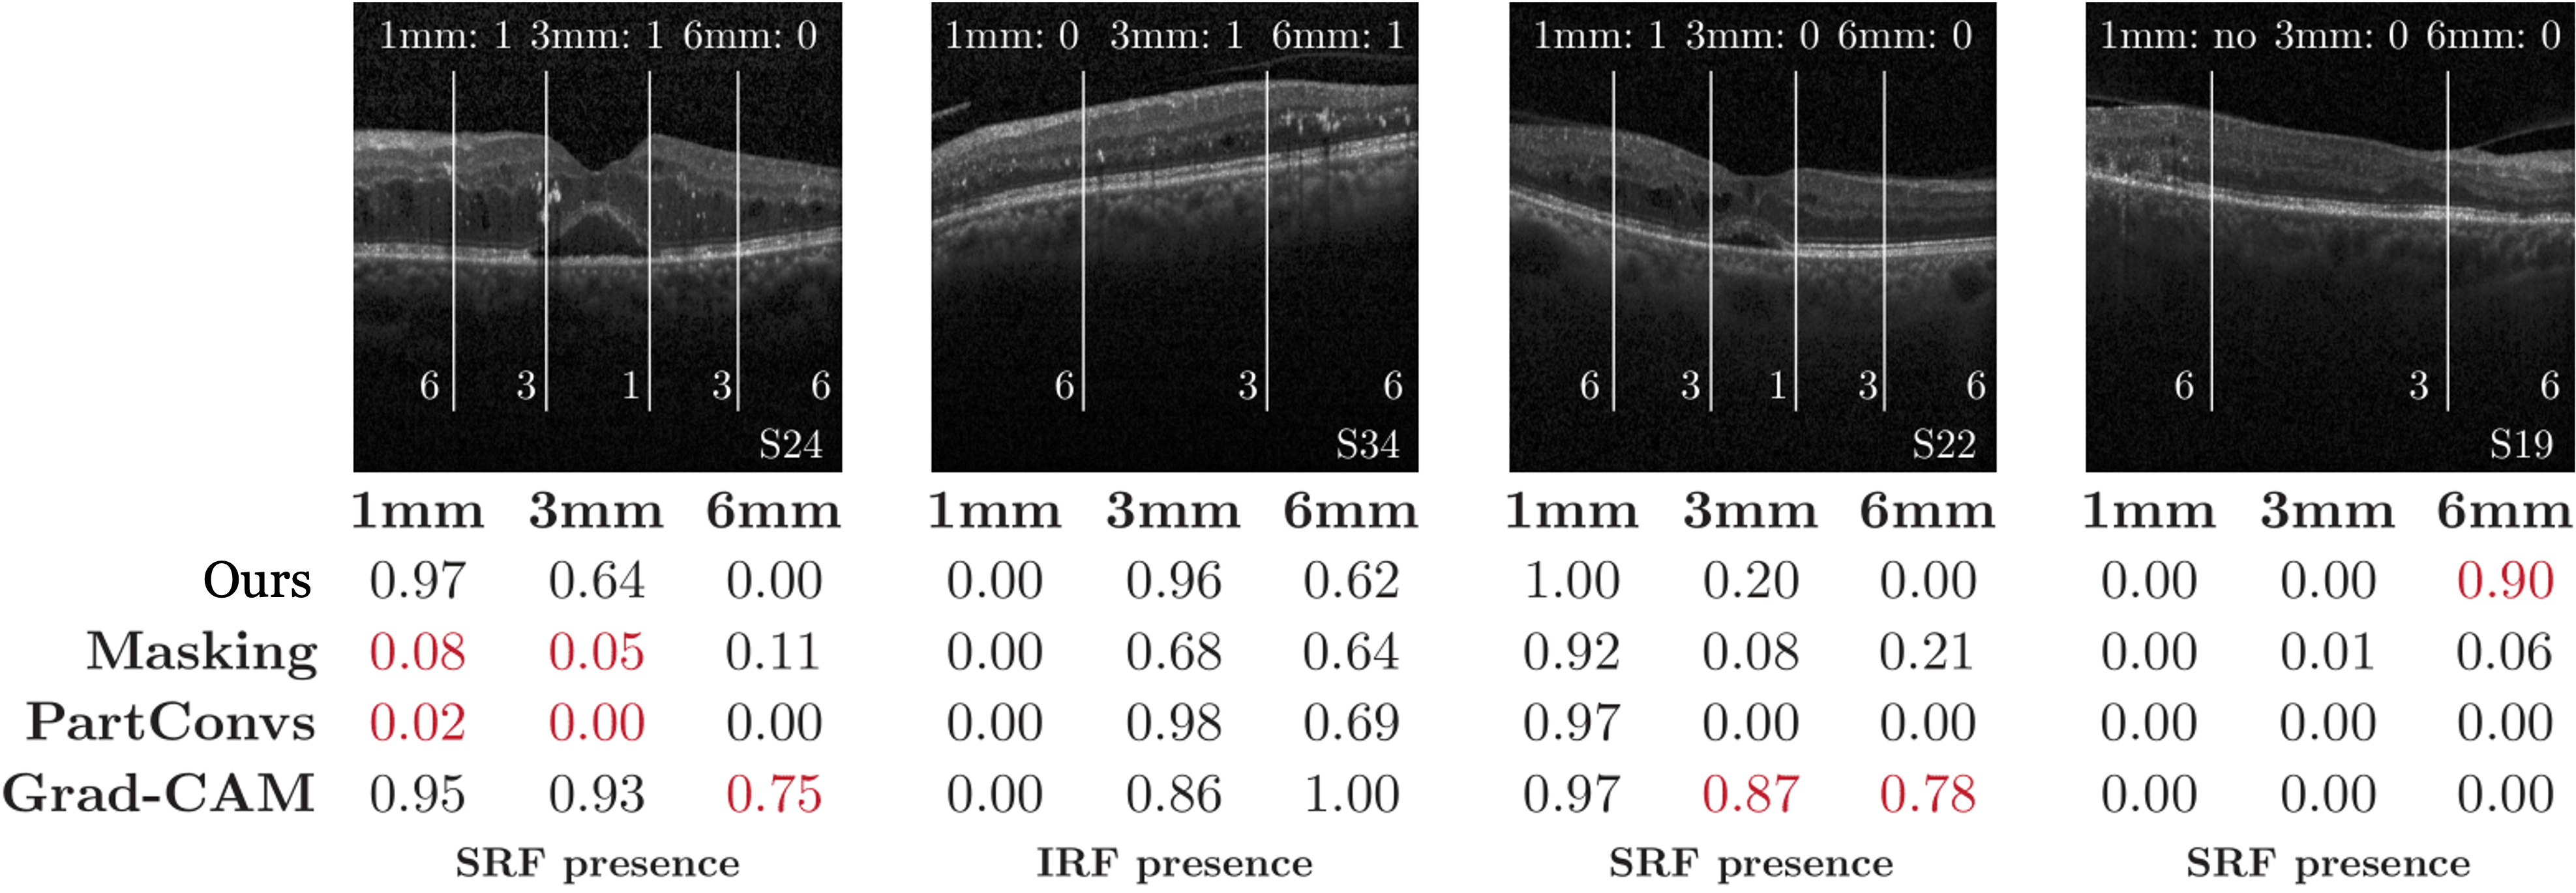
\includegraphics[width=.95\textwidth]{Figures/examples.png}
%\caption{Outputs of our method and baselines on four examples. In each OCT image, we show the slice number (bottom right) and in which ring the marker can be found (top row). We highlight incorrect detections in red.}
%\label{fig:examples}
%\end{figure}


\subsection{Segmentation results}

To further demonstrate the accuracy of our method in locating biological markers, we also compare our results to the subset of test images for which IRF and SRF ground-truth segmentations are available\sidenote{$2'646$ OCT slices}. For this purpose, a column is considered positive for a marker if it contains at least one pixel of that marker. Our method achieved AUCs over 90\% for both IRF and SRF, as shown in \Cref{tab:segmentation_results}. The low mAP for SRF can be attributed to its very low occurrence rate.

\begin{margintable}[]\small
\caption{Results on the segmentation dataset}
\label{tab:segmentation_results}
\begin{tabular}{@{}rll@{}}
\toprule
 & \textbf{IRF} & \textbf{SRF} \\ \midrule
ROC AUC & 91.1 & 93.7 \\
mAP & 81.2 & 64.8 \\ \bottomrule
\end{tabular}
\end{margintable}

\subsection{En-face projection}

Before the post-processing step that converts columns to rings, our method produces a coarse 1D segmentation per B-Scan. The projection of this output and further concatenation of all the B-Scans that compose a C-Scan results in the en-face projection.

In \Cref{tab:en_face}, we compared the coarse en-face projections that our method produces to the 54 manually segmented volumes and computed the mean area of IRF and SRF. We used a resolution of $11.72 \si{\micro\meter\per px}$ and $120 \si{\micro\meter\per slice}$ in the lateral and sagittal axes respectively. The row “Expert” refers to pixelwise segmentations, and ``16 column Expert" has been calculated by converting the pixelwise segmentation into columns, with the same methodology as in the previous section. We believe ``16 column Expert" version is a fairer comparison because it provides the same amount of information as our predictions. For IRF, we obtain a mean area of $5.73 \si{\milli\meter^2}$, being $6.29 \si{\milli\meter^2}$ the ground truth with 16 columns. For SRF, this number is less representative since only 25 of the 54 volumes contain this type of fluid.

\begin{table}[]
\centering
\begin{tabular}{@{}lll@{}}
\toprule
 & \textbf{IRF (\si{\milli\meter^2})} & \textbf{SRF (\si{\milli\meter^2})} \\ \midrule
Expert & $3.15\pm2.97$ & $0.21\pm0.63$ \\
16 column Expert & $6.29\pm4.93$ & $0.35\pm0.89$ \\
Predicted & $5.73\pm5.71$ & $0.12\pm0.30$ \\
MSE: Predicted vs 16 column Expert & $3.89\pm8.90$ & $0.46\pm2.11$ \\ \bottomrule
\end{tabular}
\sidecaption{En-face projection results. \label{tab:en_face}}
\end{table}

\Cref{fig:areas} shows the comparison of the predicted area per volume (blue) and the area delimited by the expert (red). Both figures have been calculated using the column system. \Cref{fig:en_face_qualitative} shows qualitative results of four of the volumes. Here, we compare the expert en-face projection with full segmentation (c) and after column conversion (d) to our prediction (b). 

\textfig{1}{Figures/area_columns.pdf}{Expert (red) and predicted (blue) area for IRF and SRF in each one of the 54 volumes. Blue (red) vertical lines refer to overestimations (underestimations) of our model with respect to the Expert segmentation. Volumes are sorted in decreasing order of SRF area discrepancy, and that sorting is kept for IRF.}{fig:areas}

%\begin{figure}[htbp]
%\centering
%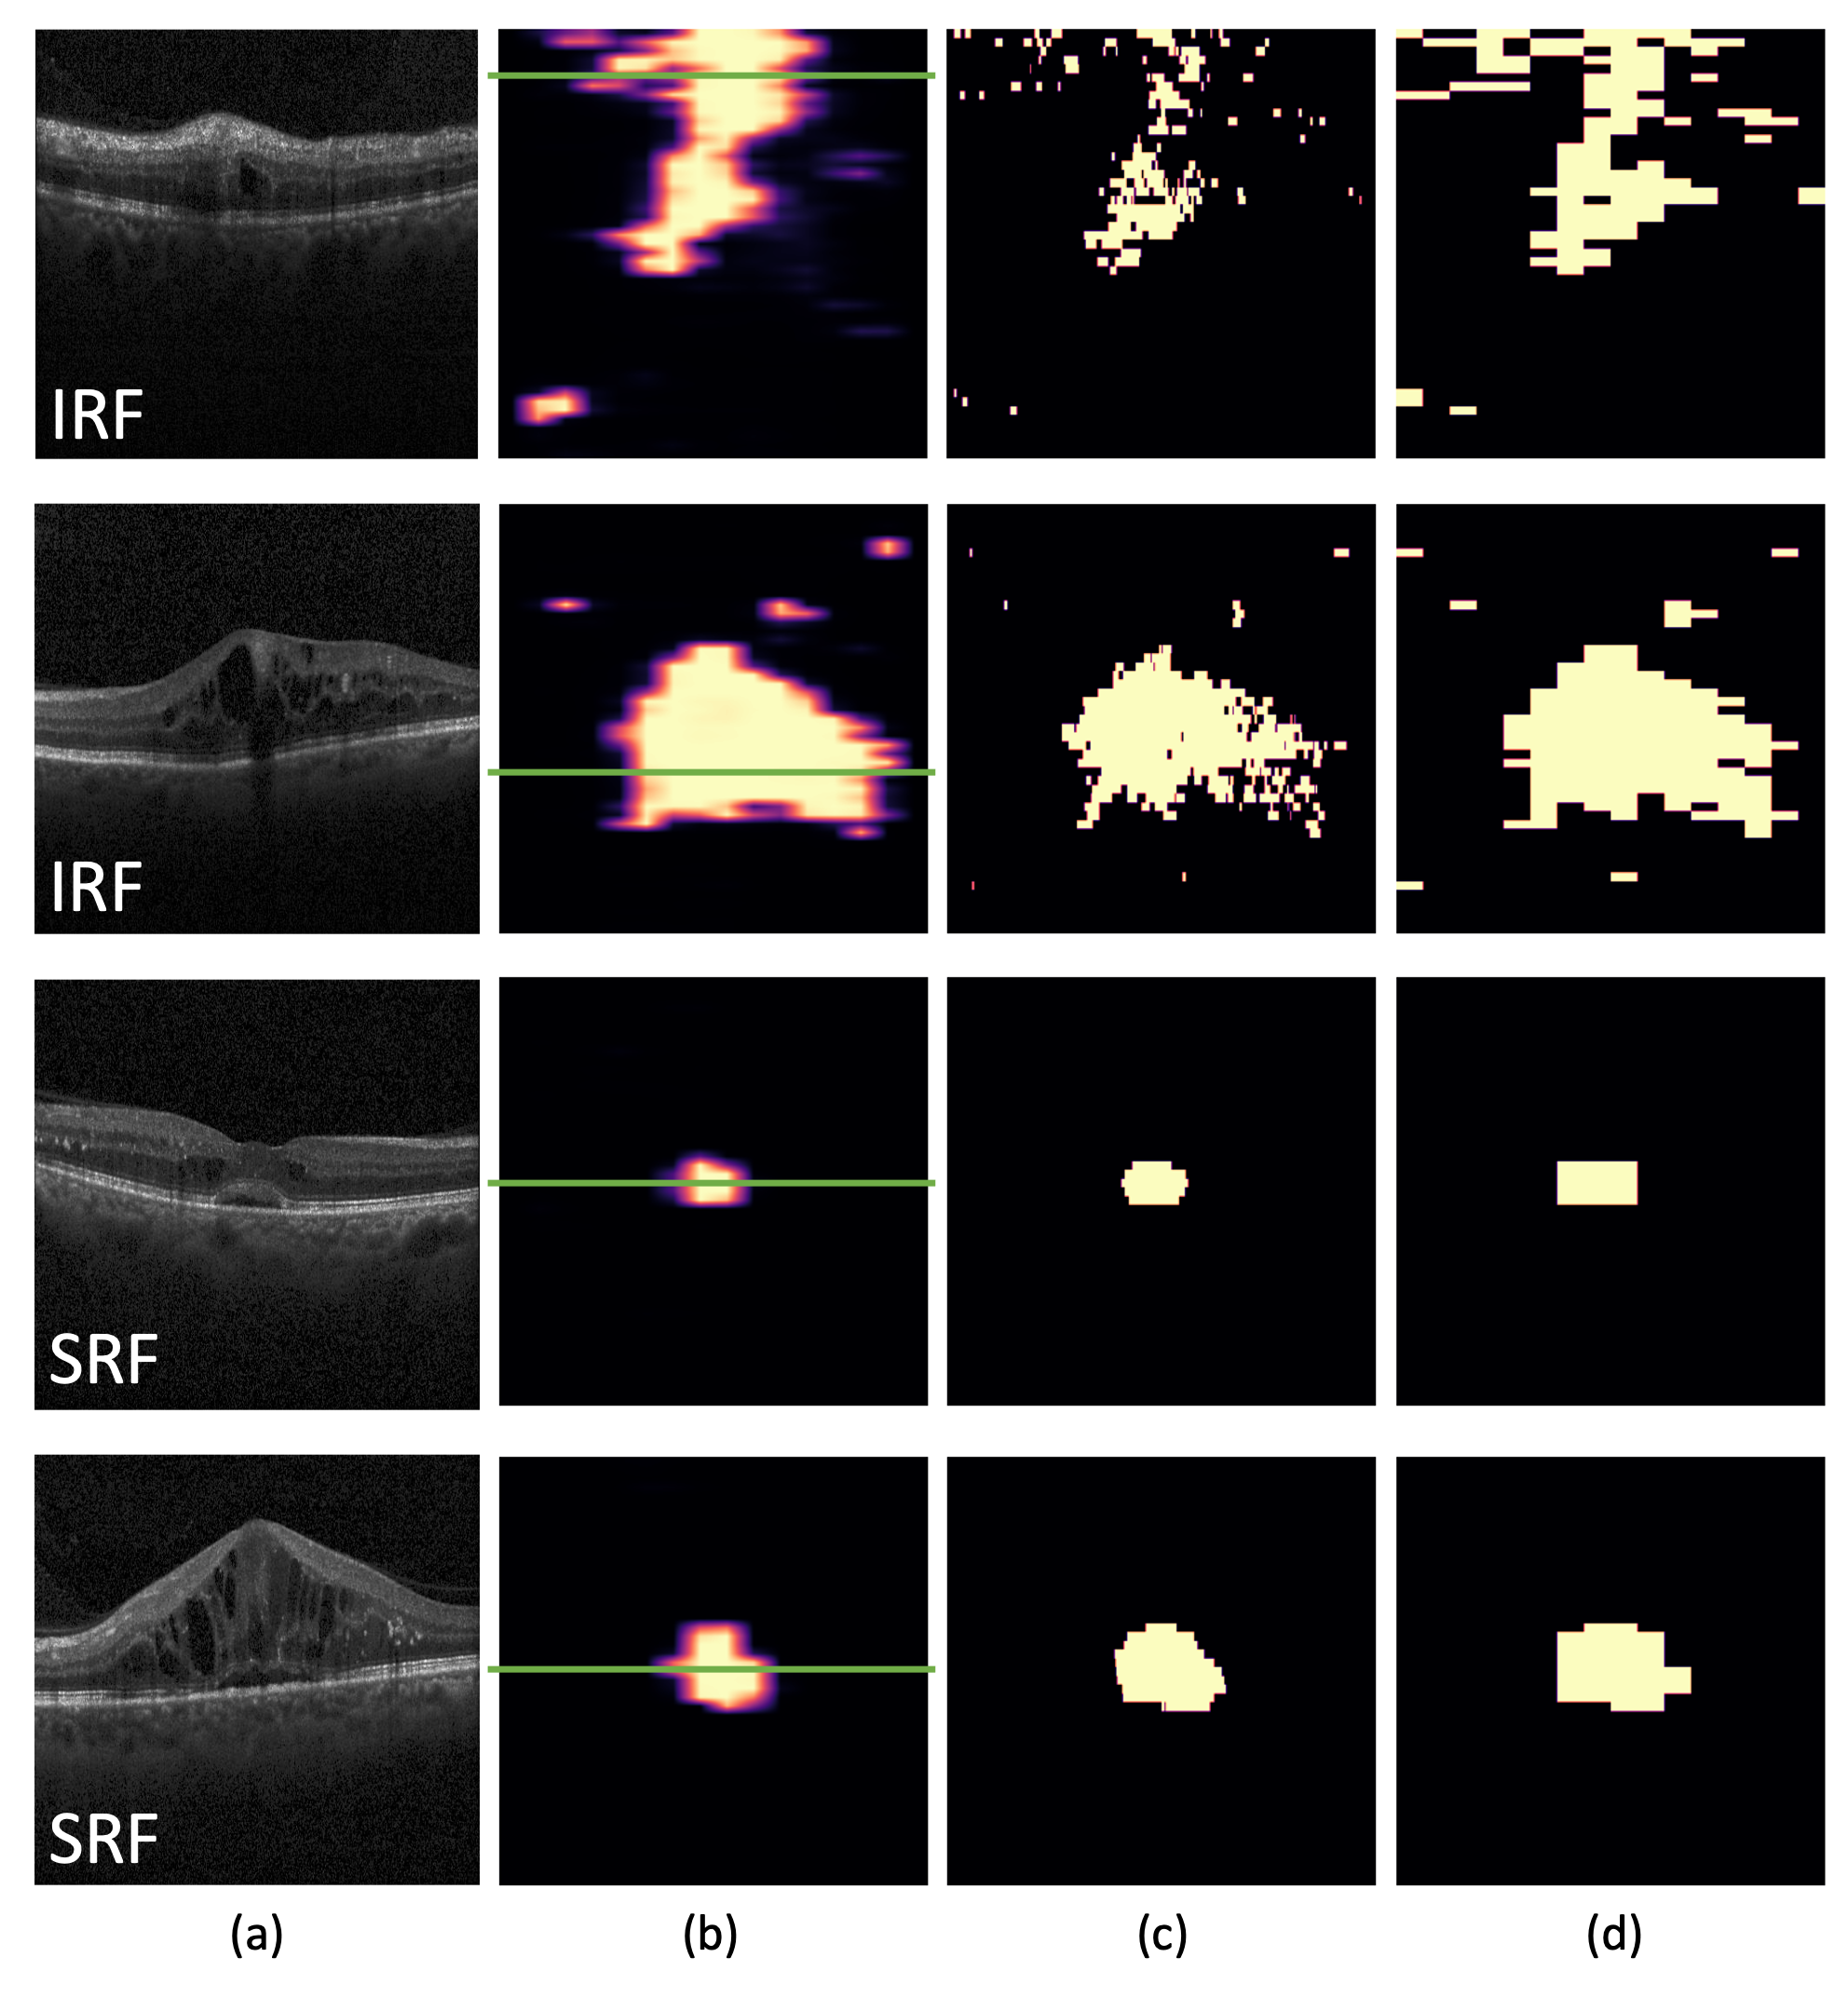
\includegraphics[width=.7\textwidth]{Figures/en_face.png}
%\caption{En-face projection results for the specified markers. (a) B-Scan at the location in green. (b) Prediction with our method. Different colors represent the uncertainty of the model. Lighter means more certain. (c) Expert pixelwise segmentation. (d) Expert segmentation converted into columns. Figure best seen in color.}
%\label{fig:en_face_qualitative}
%\end{figure}

\textfig{1}{Figures/en_face.png}{En-face projection results for the specified markers. (a) B-Scan at the location in green. (b) Prediction with our method. Different colors represent the uncertainty of the model. Lighter means more certain. (c) Expert pixelwise segmentation. (d) Expert segmentation converted into columns. Figure best seen in color.}{fig:en_face_qualitative}

To assess the clinical relevance of our method, understood as the agreement between our approach and an expert-based segmentation, we built Bland-Altman plots for SRF and IRF segmentations. In \Cref{fig:bland_altman}, we compared our prediction for the coarse en-face segmentation to the 16-column Expert in each volume. We see that four volumes fall outside one standard deviation for IRF, while only two in the case of SRF.

\Cref{fig:correlation} shows correlation plots for both biomarkers. For IRF, the linear regression returns $R^2=0.895$ and a slope close to identity (1.09). On the contrary, for SRF our method achieves $R^2=0.760$ and a slope of 0.30.

%\begin{figure}[htbp]
%\centering
%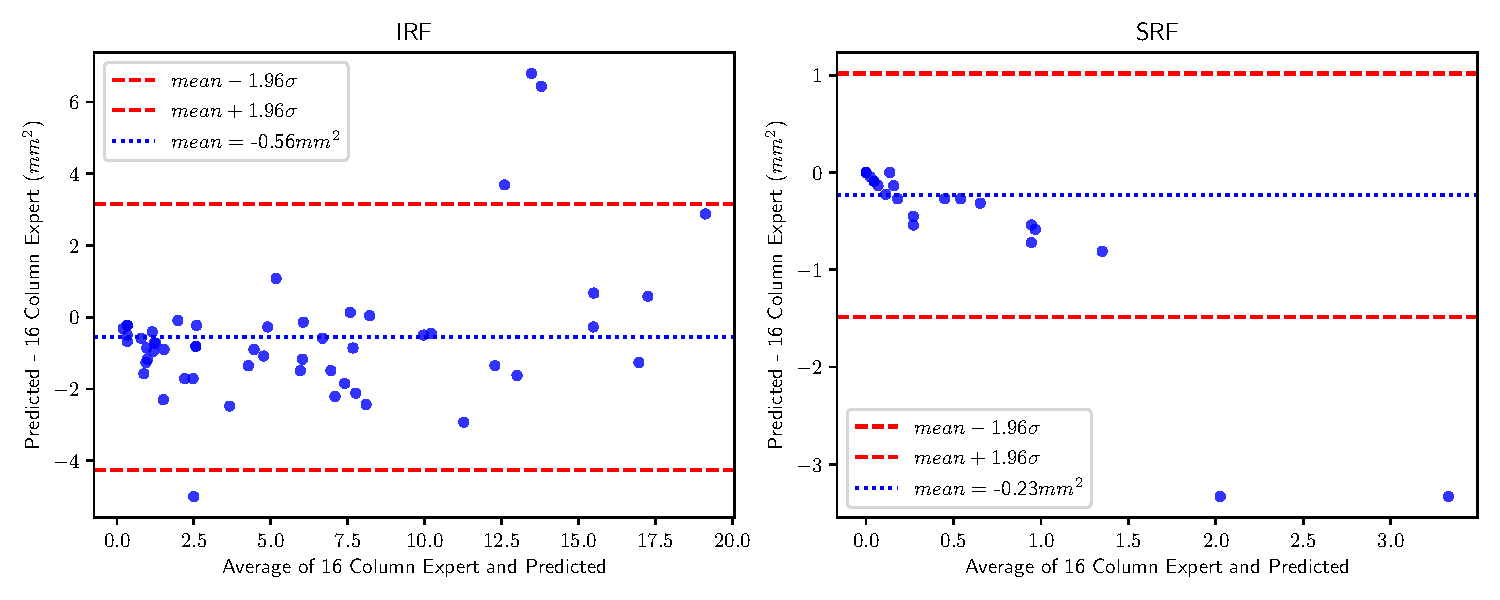
\includegraphics[width=.95\textwidth]{Figures/bland_altman.pdf}
%\caption{Bland-Altman plots for IRF and SRF}
%\label{fig:bland_altman}
%\end{figure}

\plainwidefig{1}{Figures/bland_altman.pdf}{Bland-Altman plots for IRF and SRF}{fig:bland_altman}

%\begin{figure}[htbp]
%\centering
%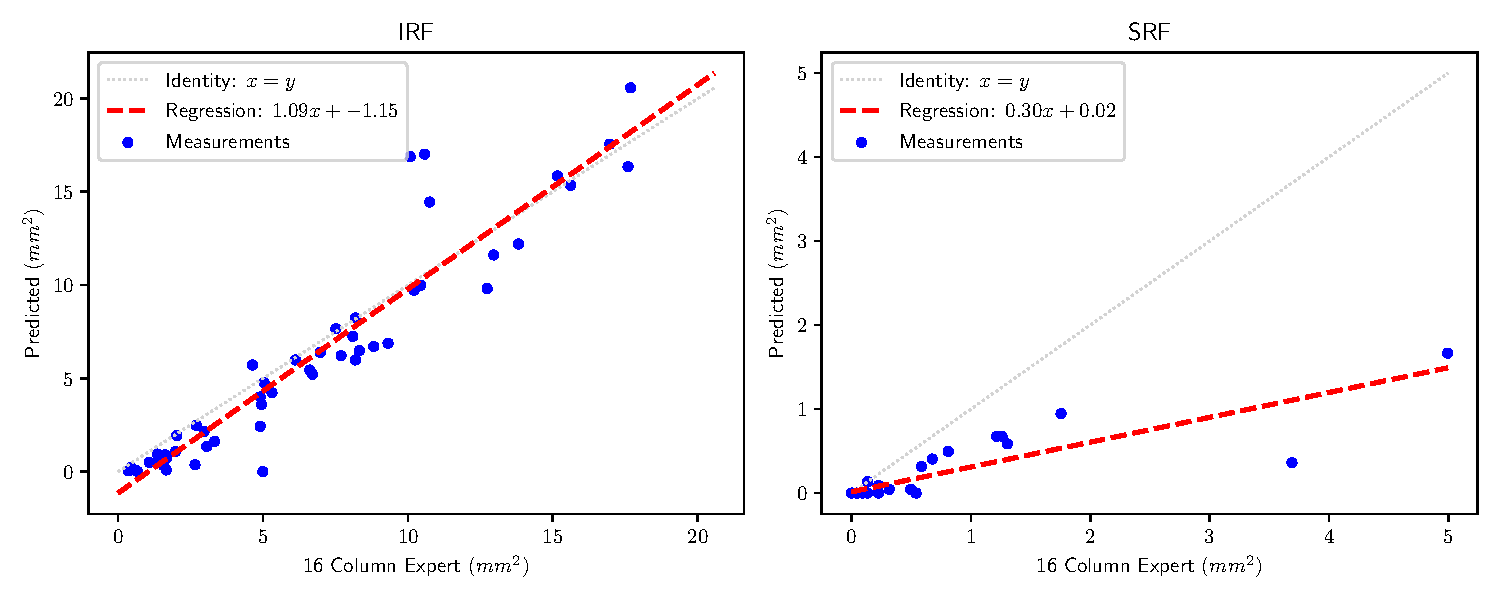
\includegraphics[width=.95\textwidth]{Figures/correlation.pdf}
%\caption{Correlation plots for IRF and SRF}
%\label{fig:correlation}
%\end{figure}

\plainwidefig{1}{Figures/correlation.pdf}{Correlation plots for IRF and SRF}{fig:correlation}

\subsection{Ablation results}
We conduct an ablation study to quantify how the different loss terms in Equation 5 affect the method's performance. \Cref{tab:ablation_loc} shows the AUC ROC and AP of all predicted outputs as a function of what loss terms are included when training. The first and fourth rows, labeled with $l_1$, correspond to using the traditional Cross Entropy loss, which does not make use of any column constraint. $l_2$ and $l_3$ do impose these constraints as described in Method. On average, there is an improvement of 5.4\% ROC AUC (18.0\% AP) after the addition of column constraints, which is further increased to 7.6 and 19.1\%, respectively, with horizontal symmetry.

\begin{table*}[t]
\centering
\caption{Ablation study. We quantify the performance of our method when using only the terms \{$\ell_1$\}, \{$\ell_1$, $\ell_2$\} or \{$\ell_1$, $\ell_2$, $\ell_3$\} in our loss functions.\label{tab:ablation_loc}}
\begin{tabular}{@{}TrSSSSSS|SS@{}}
\cmidrule(l){3-10}
\multicolumn{1}{l}{} &  & \multicolumn{2}{c}{\textbf{1mm}} & \multicolumn{2}{c}{\textbf{3mm}} & \multicolumn{2}{c}{\textbf{6mm}} & \multicolumn{2}{c}{\textbf{Present}} \\ \cmidrule(l){3-10} 
\multicolumn{1}{l}{} &  & \multicolumn{1}{c}{\textbf{IRF}} & \multicolumn{1}{c}{\textbf{SRF}} & \multicolumn{1}{c}{\textbf{IRF}} & \multicolumn{1}{c}{\textbf{SRF}} & \multicolumn{1}{c}{\textbf{IRF}} & \multicolumn{1}{c|}{\textbf{SRF}} & \multicolumn{1}{c}{\textbf{IRF}} & \multicolumn{1}{c}{\textbf{SRF}} \\ \midrule
\multirow{3}{*}{\textbf{AUC}} & \multicolumn{1}{l|}{$\ell_1$} & 88.0 & 90.7 & 90.2 & 81.9 & 92.6 & \multicolumn{1}{l|}{73.7} & 96.5 & 96.2 \\
 & \multicolumn{1}{l|}{$\ell_1, \ell_2$} & 87.8 & 96.9 & 90.1 & 92.3 & 92.2 & \multicolumn{1}{l|}{91.7} & 96.5 & 95.9 \\
 & \multicolumn{1}{l|}{$\ell_1, \ell_2, \ell_3$} & \textbf{90.6} & \textbf{97.5} & \textbf{92.7} & \textbf{93.8} & \textbf{94.1} & \multicolumn{1}{l|}{\textbf{95.1}} & \textbf{97.2} & \textbf{97.7} \\ \midrule
\multirow{3}{*}{\textbf{AP}} & \multicolumn{1}{l|}{$\ell_1$} & 91.5 & 71.4 & 91.7 & 29.4 & 85.8 & \multicolumn{1}{l|}{13.8} & 96.1 & 72.3 \\
 & \multicolumn{1}{l|}{$\ell_1, \ell_2$} & 90.9 & 84.8 & 91.7 & 41.5 & 86.5 & \multicolumn{1}{l|}{\textbf{24.4}} & 96.3 & 77.1 \\
 & \multicolumn{1}{l|}{$\ell_1, \ell_2, \ell_3$} & \textbf{92.1} & \textbf{86.6} & \textbf{93.7} & \textbf{52.7} & \textbf{88.3} & \multicolumn{1}{l|}{19.1} & \textbf{96.8} & \textbf{77.9} \\ \bottomrule
\end{tabular}

\end{table*}